\section{Ingestion-Service}
\label{sec:entw-ingestion}

Der Ingestion-Service hat die Aufgabe den Spark-Job für die Ausführung einer Ingestion zu erstellen, zu starten und zu überwachen und den Status des IngestionEvents anzupassen.
Dazu gehört das Festlegen des Ablaufs zum Laden der Daten in ein DataFrame, zur Deltaberechnung und zum Speichern.
Ein zweiter wichtiger Teil ist die Integration der Plugins in den Ingestion-Prozess.
Ebenfalls koordiniert der Ingestion-Service die parallele Ausführung von Ingestions.

Der Ingestion-Service wartet auf die Nachricht zur Ausführung einer Ingestion, mit der Id der DatasourceDefinition.
Als erstes wird geprüft, ob bereits eine Ingestion der Datenquelle aktiv ist.
Falls das nicht der Fall ist, wird ein neuer Prozess gestartet, indem die Ingestion ausgeführt wird.
Auf diese Art wird die Parallelität ermöglicht.

Der Ablauf einer Ingestion kann unabhängig vom Lese- und Schreib-Typ in einem allgemeinen Ablauf, wie in \cref{fig:ingestion-ablauf}, abgebildet werden.
Als erstes wird die Ingestion vorbereitet.
Hier werden die Plugins und deren Abhängigkeiten installiert und eine SparkSession erstellt.
Im nächsten Schritt werden die Daten aus der Quelle geladen.
Wenn es sich dabei um Ändeurngsdaten aus einer Updatequelle handelt, können diese direkt in den entsprechenden Zieldatensatz eingepflegt werden.
Ist das nicht der Fall, folgt eine Entscheidung, ob Änderungsdaten berechnet werden müssen.
Es gelten die folgenden zwei Regeln: \begin{itemize}
    \item der Speicher-Typ ist Delta und
    \item es ist nicht die erste Ingestion dieser Datenquelle.
\end{itemize}
Wurden Änderungsdaten berechnet, werden diese eingepflegt.
Wurden keine berechnet, werden die Daten einfach gespeichert.
Ist das Speicherziel dabei ein Delta Tabelle wird diese angelegt und ist es eine Parquet-Datei, dann werden die aktuellen Daten überschrieben.
Handelt es sich nicht um einen benutzerdefinierten Speicher, werden die alten Daten mit den neuen überschrieben.

\begin{figure}
    \centering
    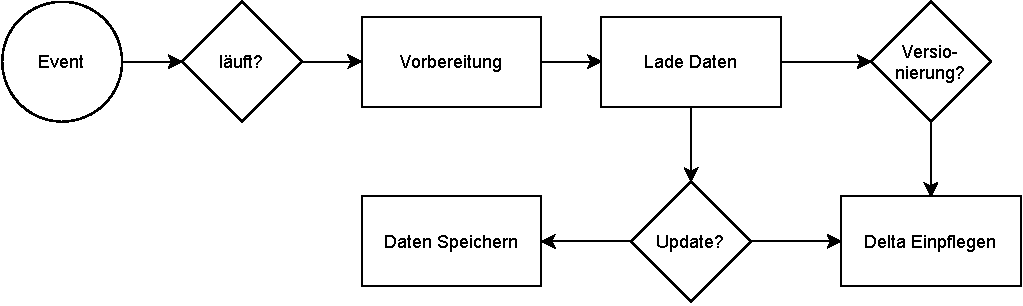
\includegraphics[width=\textwidth]{Grafiken/Entwicklung-Ingestion-Ablauf.pdf}
    \caption{Ablauf einer Ingestion}
    \label{fig:ingestion-ablauf}
\end{figure}